\begin{frame}[fragile]{Using UHD from Python (4/7)}

\footnotesize

\begin{itemize}
    \item \textbf{\textcolor{DarkBlue}{Step 4: Basic Python Program for Receiving IQ Samples}}
\end{itemize}

\hspace{2.8em}
\parbox{0.88\linewidth}{
The following example demonstrates a Python application that receives IQ
samples from a USRP B210 using the UHD Python API and stores the captured
samples in a NumPy (\texttt{.npy}) file.
}

\vspace{0.3cm}

\begin{columns}[T]

%================ Left Column ===================
\column{0.45\textwidth}

\footnotesize
\textbf{Program Flow}

\vspace{0.15cm}

\begin{itemize}
    \item Parse command-line arguments
    \begin{itemize}
        \scriptsize
        \item Output filename
        \item Frequency
        \item Sample rate
        \item Capture duration
        \item Gain
    \end{itemize}

    

    \item Create a \texttt{MultiUSRP} object.

    

    \item Configure receiver parameters.

   

    \item Receive IQ samples from the USRP.

   

    \item Save the received samples into a
    \texttt{.npy} file.
\end{itemize}

%================ Right Column ===================
\column{0.55\textwidth}

\centering
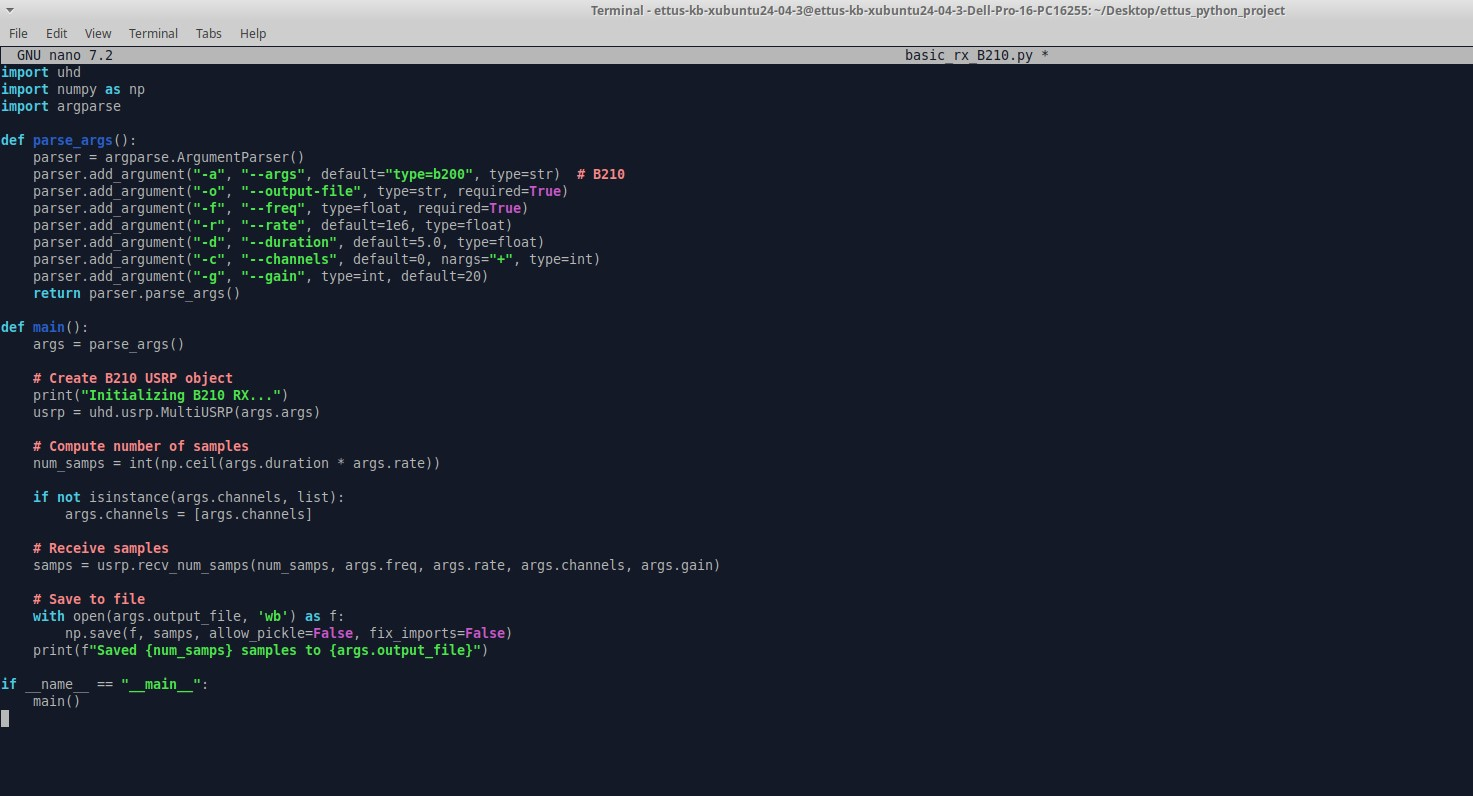
\includegraphics[
width=\linewidth,
height=0.63\textheight,
keepaspectratio]
{latex/jpg_png/image_python_api_basic rx code B210.jpg}

\end{columns}

\end{frame}